\begin{itemize}
	\item The operational block diagrams of a digital system
	in the various canonical forms is shown in the final sequence of
	slides.
\end{itemize}
\begin{slide}\label{slide:l9s14}
\heading{Controller Canonical Form}
\resizebox{300pt}{!}{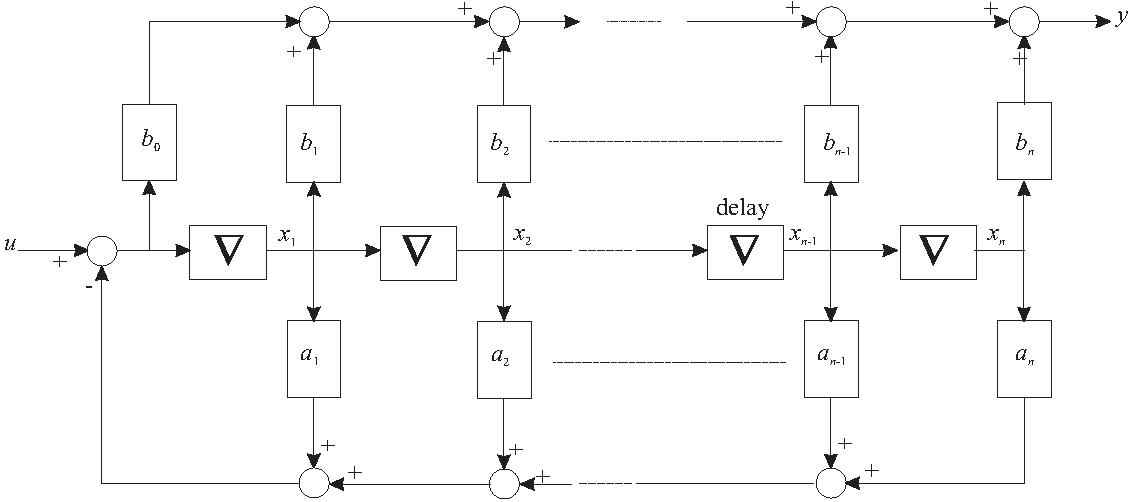
\includegraphics{pictures/dccanon.pdf}}
\end{slide}

\begin{slide}\label{slide:l9s15}
\heading{Observer Canonical Form}
\resizebox{300pt}{!}{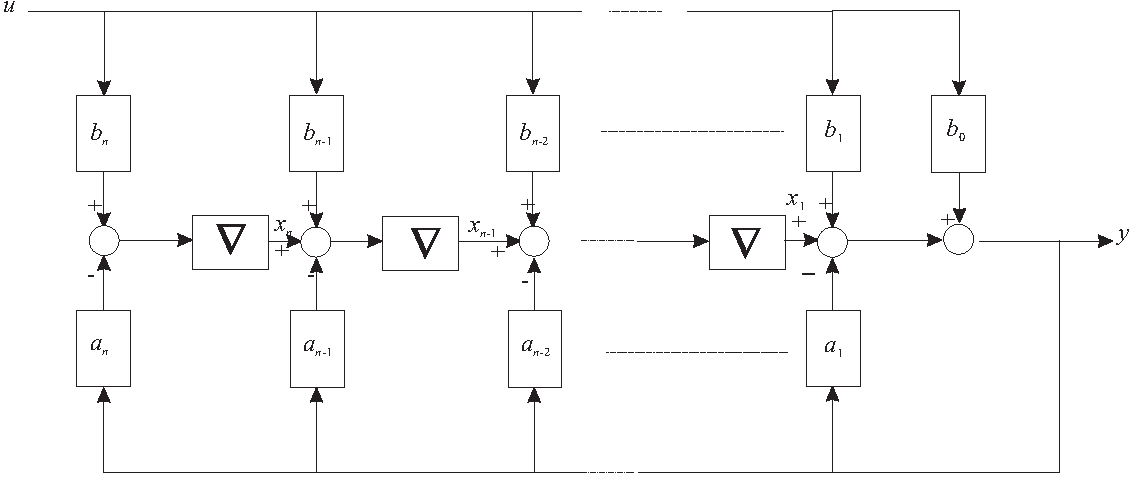
\includegraphics{pictures/docanon.pdf}}
\end{slide}

\begin{slide}\label{slide:l9s16}
\heading{Normal Canonical Form}
\resizebox{300pt}{!}{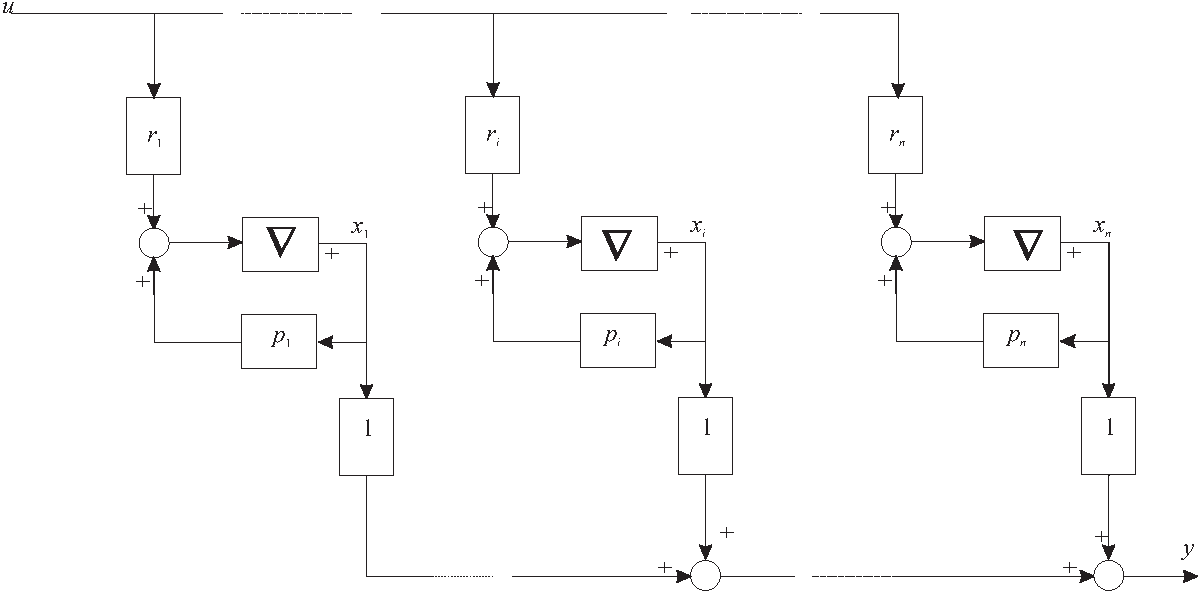
\includegraphics{pictures/dnrmlcan.pdf}}
\end{slide}

In the next lecture we will consider the system response of
systems represented by digital transfer functions.
